\section{Joint atmospheric and persistent calibration robustness}
Let $B$ contain the 54 previously archived atmospheric discrepancy spectra. We now declare the mean-error set
\[
\mathcal B=\operatorname{conv}\{\pm b_s:1\le s\le54\}
+\{u:\|u\|_\infty\le\epsilon\}.
\]
The first component represents the finite atmospheric design envelope; the second is a persistent per-frequency calibration error, not independent noise that averages down with pilots. Neither component is an empirically calibrated confidence region. For a row $h^T$ satisfying $h^TD=e_j^T$ and $h^TN=0$, its exact worst squared error under diagonal variance $v$ is
\begin{equation}
R_j^2(h)=\sum_i v_i h_i^2+
\left(\max_s|h^Tb_s|+\epsilon\|h\|_1\right)^2.
\label{eq:joint-risk}
\end{equation}
The support function of the symmetric finite hull is $\max_s|h^Tb_s|$; the box support is $\epsilon\|h\|_1$. Their sum is attained independently, which proves (\ref{eq:joint-risk}). Worst cases for different gases need not be the same physical state. Minimizing this convex objective over the equality constraints gives the calibration-aware linear estimator. We retain the complete equality nullspace, because restricting it to the span of atmospheric errors can miss directions relevant to the $\ell_1$ penalty. This is a specialization of convex robust estimation, not a new general optimization principle.

The grid uses $\epsilon=0,10^{-5},10^{-4},10^{-3}$ dB, independent random residual SD 0 or .001 dB, and eight acquisition scenarios. Every comparison with the atmospheric-only estimator uses the same variance, probes and error envelope. All 128 estimator/scenario combinations complete and produce 512 gas summaries. Their design objective is no worse than the atmospheric-only control within solver tolerance. We replay the 64 previously inspected atmospheric states, adding the same targetwise calibration worst case; this continuation does not call those states a new independent validation set.

\begin{figure*}[t]\centering
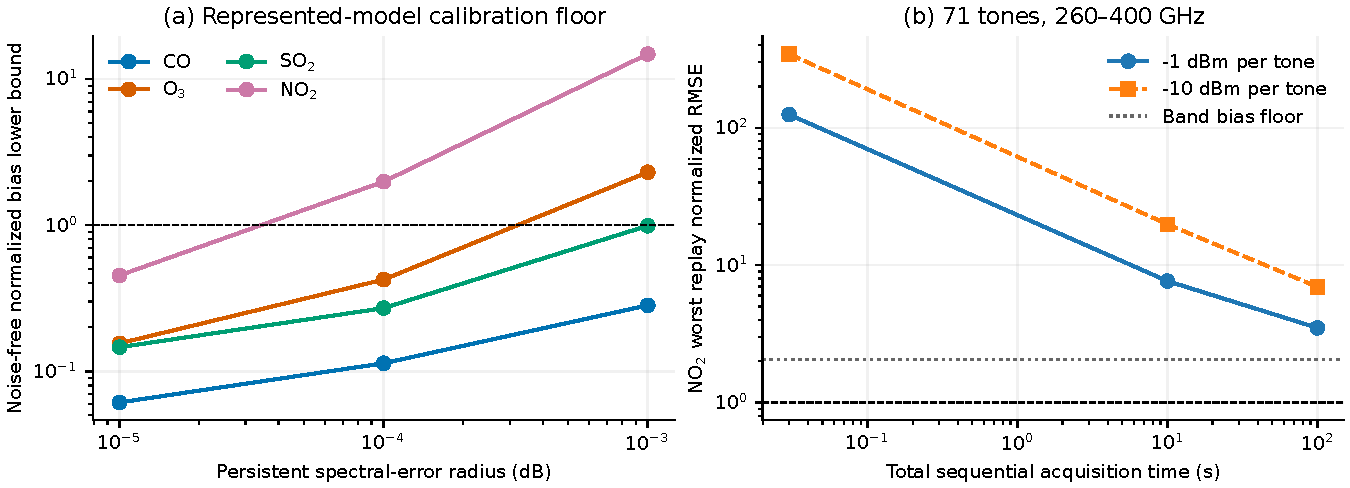
\includegraphics[width=.9\textwidth]{../results/continuation_calibration/calibration_limits.pdf}
\caption{Left: exact represented-LP dual lower bounds with all 202 probes. Right: NO$_2$ stress-replay RMSE at $10^{-4}$ dB persistent error, zero random residual and sequential band acquisition. The unit line is the declared magnitude-normalized error target. These are conditional calculations, not measured gas retrieval.}
\end{figure*}

\section{A resource-independent calibration floor}
Even if thermal noise vanishes, every estimator in this unbiased linear class has worst RMSE at least
\begin{equation}
\phi_j(\epsilon)=\min_{h^TD=e_j^T,\,h^TN=0}
\left\{\max_s|h^Tb_s|+\epsilon\|h\|_1\right\}.
\label{eq:bias-floor}
\end{equation}
Split $h=h^+-h^-$ with nonnegative parts and introduce $t\ge\pm b_s^Th$. This is a linear program with objective $t+\epsilon\mathbf1^T(h^++h^-)$. For its stored normalized equality matrix $A_E$, inequality matrix $A_U$, right-hand side $d_E$ and positive cost $c$, any exact rational vectors satisfying
\[
\mu\le0,\qquad A_E^T\lambda+A_U^T\mu\le c
\]
give the lower bound $d_E^T\lambda$ by weak duality. The implementation clips inequality duals to the correct sign and scales both dual vectors until every inequality holds in exact rational arithmetic. The serialized coefficient arrays, rational vectors and a separate verifier make all 24 bounds machine checkable. Numerical primal/dual gaps are below $9.3\times10^{-11}$.

\begin{table}[t]\centering\scriptsize
\caption{Rounded displays of certified lower bounds on noise-free normalized worst bias, all 202 probes. Certificates apply to the represented normalized LP coefficients.}
\begin{tabular}{rrrrr}\toprule
$\epsilon$ [dB] & CO & O$_3$ & SO$_2$ & NO$_2$\\\midrule
$10^{-5}$ & 0.061 & 0.155 & 0.146 & 0.453\\
$10^{-4}$ & 0.113 & 0.424 & 0.270 & 1.984\\
$10^{-3}$ & 0.283 & 2.303 & 0.990 & 14.806\\
\bottomrule\end{tabular}

\end{table}
At $\epsilon=10^{-4}$ dB, the NO$_2$ lower bound is 1.9837335 with all probes and 2.0556340 in the 260--400 GHz band. Thus the declared four-gas error target cannot hold over this envelope for any estimator in the represented unbiased linear model, irrespective of pilot count. This is a conditional impossibility result for that model class and envelope. It is not a physical interval certificate for spectroscopy, a measured receiver limitation, or an impossibility theorem for nonlinear or prior-assisted retrieval. Bounds below one do not by themselves establish feasibility with noise.

\section{Sequential acquisition and finite-resource results}
A published VDI extender table lists a 260--400 GHz test-port band and typical output of $-1$ dBm; its dated March 2022 summary lists $-10$ dBm for that band~\cite{vdiCurrent,vdi2022}. We retain both powers as scenarios. Typical magnitude stability of $\pm.5$ dB in the current table is neither a measured spectral error for our setup nor the random residual SD in our likelihood. Dynamic range is also not used as an estimation precision specification.

The band contains 71 archived probes. With one tone at a time, pilot duration $T_s=1\,\mu$s, total duration $T$ and inter-tone retuning time $t_r$, equal dwell permits
\[
N_p=\left\lfloor\frac{T-70t_r}{71T_s}\right\rfloor.
\]
At zero retuning, 30 ms, 10 s and 100 s give 422, 140,845 and 1,408,450 pilots per tone. The 10 s, $-1$ dBm case radiates .0079433 J, compared with 1.9953 J for the legacy ideal simultaneous 23 dBm allocation. Thermal variance is rescaled with tone power. The original LEO path, apertures, noise figure and coherent likelihood remain assumptions; this source specification does not demonstrate a realizable satellite receiver. Retuning sensitivities of .1, 1 and 10 ms are archived, and infeasible short sweeps are retained.

\begin{table}[t]\centering\scriptsize
\caption{Calibration-aware worst RMSE on the 64-state stress replay, $\epsilon=10^{-4}$ dB and zero independent random residual. Band rows use sequential $-1$ dBm probing; full rows retain ideal simultaneous probing.}
\begin{tabular}{lrrrr}\toprule
Acquisition & CO & O$_3$ & SO$_2$ & NO$_2$\\\midrule
Full, 30 ms & 0.290 & 1.422 & 0.809 & 12.594\\
Full, 10 s & 0.140 & 0.802 & 0.447 & 2.425\\
Band, 10 s & 0.276 & 1.328 & 0.658 & 7.654\\
Band, 100 s & 0.230 & 0.957 & 0.515 & 3.489\\
\bottomrule\end{tabular}

\end{table}
In the legacy ten-million-pilot case, calibration-aware NO$_2$ improves from 3.385 for the atmospheric-only estimator to 2.425, yet fails the unit target. The earlier all-four success at zero persistent error is therefore a special point, not a robust operating specification. At 30,000 pilots CO and SO$_2$ retain replay worst errors below one (.290 and .809), while O$_3$ and NO$_2$ do not. Longer dwell in the single band helps its noise component but cannot remove the certified bias floor.
